\section{Mesh}\label{sec:mesh}
To solve the SWEs on the sphere we need to cover the sphere with elements. A lat-lon grid seems like a good choice, but its grid lines converge at the poles, where the elements become very small and the explicit time step with them, and the poles are singular points. Instead we follow \cite{bonev2018discontinuous, GIRALDO2002499} and build a mesh of quadrilaterals from an icosahedron. It has no singular points, and all elements are roughly the same size.

\subsection{Construction}\label{sec:mesh-construction}
The mesh is built in four steps, controlled by one refinement parameter $n_I$.

\paragraph{Icosahedron}
The icosahedron has the 12 vertices $(0,\pm1,\pm\varphi)$, $(\pm1,\pm\varphi,0)$ and $(\pm\varphi,0,\pm1)$, where $\varphi = (1+\sqrt5)/2$, which we normalise to lie on the unit sphere. Its 20 faces are equilateral triangles, which we take from the convex hull of the vertices and order counter-clockwise seen from outside the sphere.

\paragraph{Subdivision}
Each face with the vertices $\mathbf{A}$, $\mathbf{B}$, $\mathbf{C}$ is divided into $n_I^2$ triangles through the points
\begin{equation*}
    \mathbf{p}_{ab} = \mathbf{A} + \frac{a}{n_I}(\mathbf{B}-\mathbf{A}) + \frac{b}{n_I}(\mathbf{C}-\mathbf{A}), \qquad a,b\in\{0,1,\dots,n_I\},\quad a+b\leq n_I
\end{equation*}

\begin{figure}[H]
    \centering
    \begin{subfigure}{0.32\textwidth}
        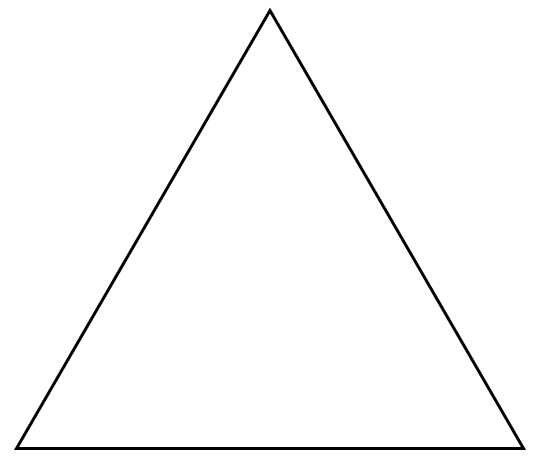
\includegraphics[width=\textwidth]{Figures/Sketches/Rough.png}
        \caption{Regular triangular face of the icosahedron}
    \end{subfigure}
    \hfill
    \begin{subfigure}{0.32\textwidth}
        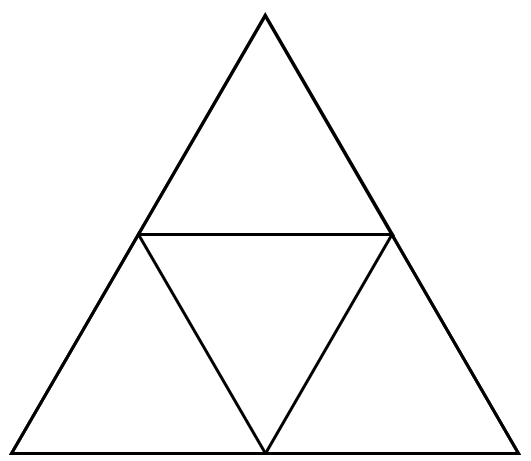
\includegraphics[width=\textwidth]{Figures/Sketches/Finer.png}
        \caption{Triangle refined to $n_I^2 = 2^2 = 4$ triangles}
    \end{subfigure}
    \hfill
    \begin{subfigure}{0.32\textwidth}
        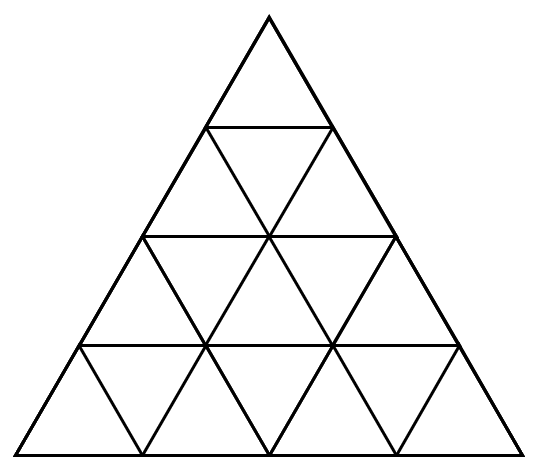
\includegraphics[width=\textwidth]{Figures/Sketches/Finest.png}
        \caption{Triangle refined to $n_I^2 = 4^2 = 16$ triangles}
    \end{subfigure}
    \caption{Refinement of the icosahedron faces}
    \label{fig:Tri_refine}
\end{figure}

\paragraph{Triangles to quadrilaterals}
Each small triangle is split into three quadrilaterals by connecting its centroid to the midpoints of its sides. Every quadrilateral has one vertex of the triangle, two midpoints and the centroid as vertices, ordered counter-clockwise. This gives
$K = 20\cdot n_I^2\cdot 3 = 60\,n_I^2 $ elements.
\begin{figure}[H]
    \centering
    \begin{subfigure}{0.48\textwidth}
        \centering
        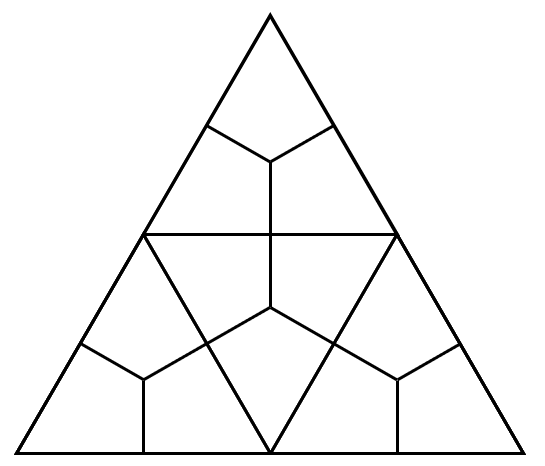
\includegraphics[width=0.5\textwidth]{Figures/Sketches/Finer_quad.png}
        \caption{4 triangles made into 12 quadrilateral elements}
    \end{subfigure}
    \hfill
    \begin{subfigure}{0.48\textwidth}
        \centering
        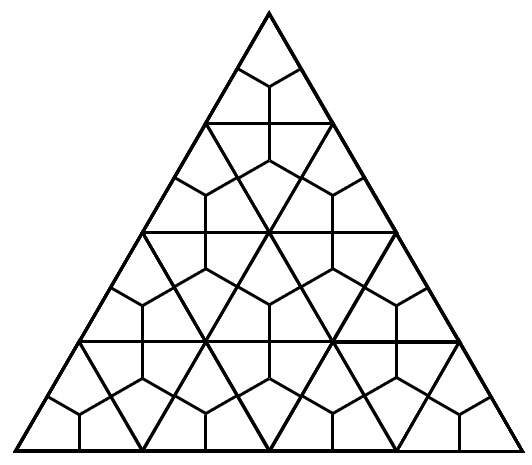
\includegraphics[width=0.5\textwidth]{Figures/Sketches/Finest_Quad.png}
        \caption{16 triangles made into 48 quadrilateral elements}
    \end{subfigure}
    \caption{Splitting different refinement levels into quads}
    \label{fig:Quads}
\end{figure}


\paragraph{Projection and merging}
The vertices are projected radially onto the sphere, $\mathbf{v}\mapsto\mathbf{v}/|\mathbf{v}|$. Since the elements are generated triangle by triangle, a vertex shared by several elements is generated several times. We merge points closer than $10^{-10}$ (using a $k$-d tree), which gives the vertex list \texttt{VX} and the element-to-vertex table \texttt{EToV}. Only the vertices are projected onto the sphere here; the curved elements between them are defined by the mapping in section \ref{sec:dg-grid}.

\begin{figure}[H]
    \centering
    \begin{subfigure}{0.48\textwidth}
        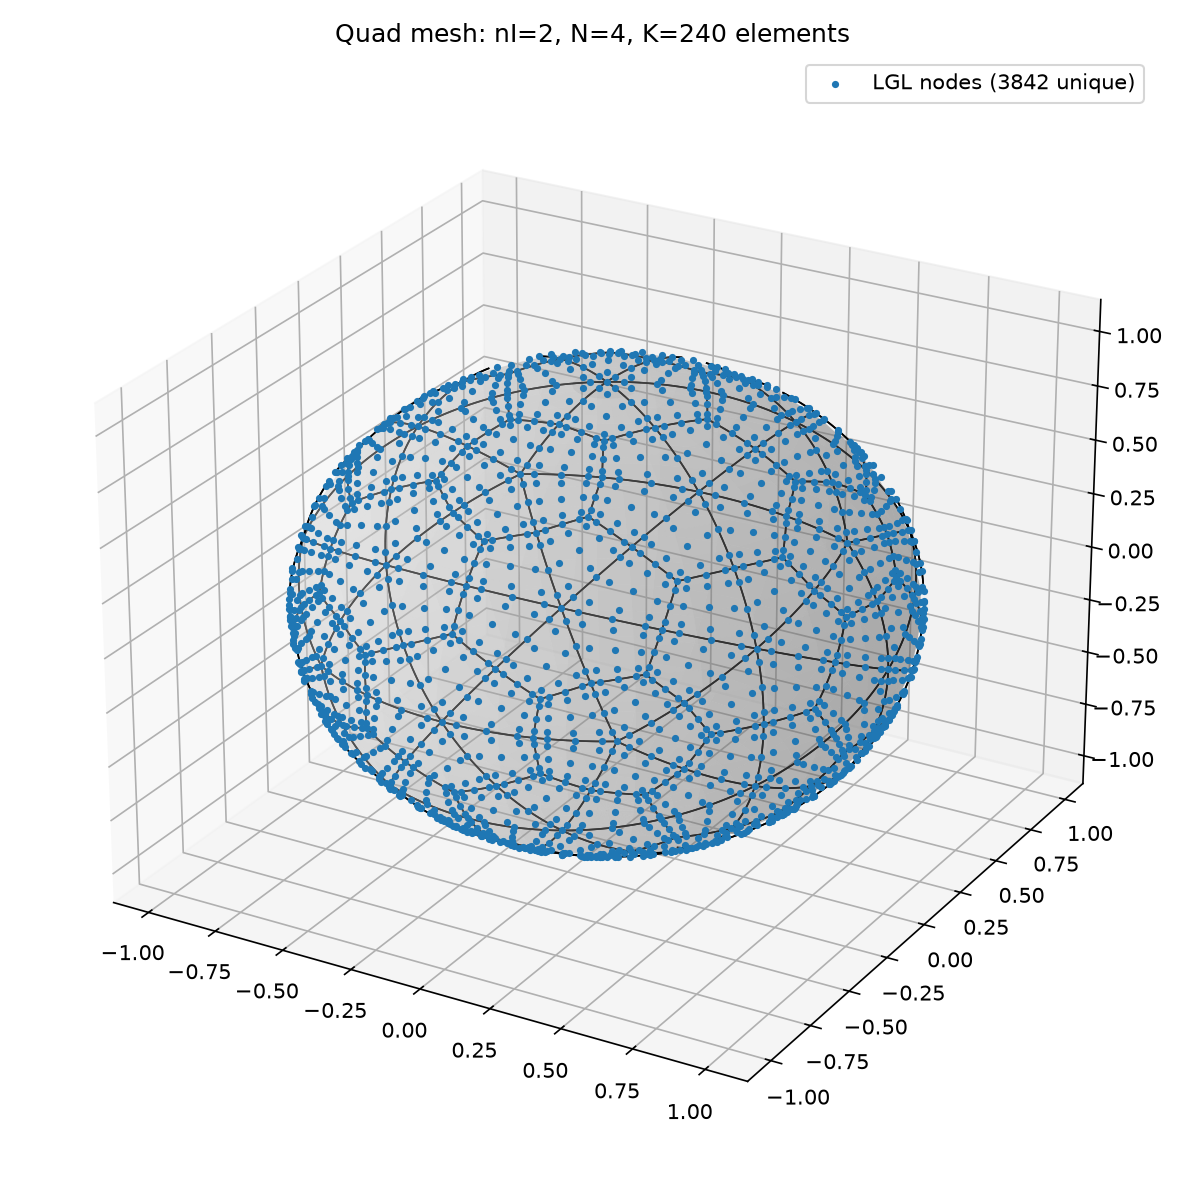
\includegraphics[width=\textwidth]{Figures/mesh_nI2_N4_K240.png}
        \caption{$n_I = 2$, $K = 240$}
    \end{subfigure}
    \hfill
    \begin{subfigure}{0.48\textwidth}
        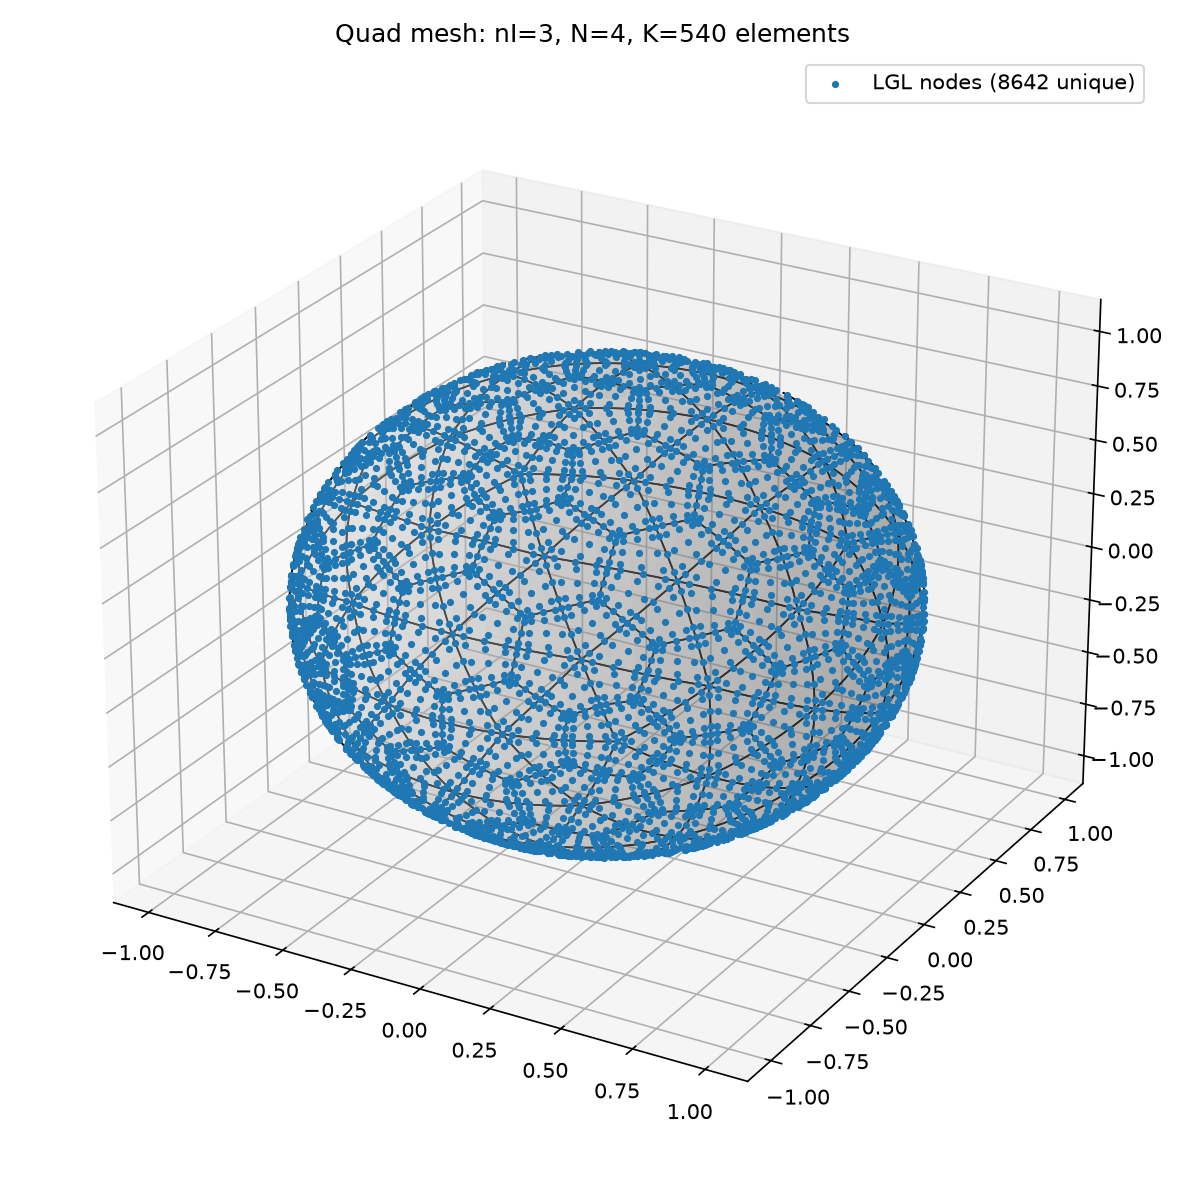
\includegraphics[width=\textwidth]{Figures/mesh_nI3_N4_K540.png}
        \caption{$n_I = 3$, $K = 540$}
    \end{subfigure}
    \caption{The icosahedral mesh with the curved elements and the LGL nodes for $N = 4$. Only the hemisphere facing the viewer is shown.}
    \label{fig:mesh}
\end{figure}

\subsection{Connectivity}\label{sec:mesh-connectivity}
The DG scheme only couples neighbouring elements through their shared sides (section \ref{sec:dg-flux}), so we need to know, for every side of every element, which element is on the other side. Side $f = 0,1,2,3$ of element $e$ runs between the local vertices $(0,1)$, $(1,2)$, $(2,3)$ and $(3,0)$. We store
\begin{itemize}
    \item \texttt{EToV}$(e,i)$: the global number of local vertex $i$ of element $e$,
    \item \texttt{EToE}$(e,f)$: the element on the other side of side $f$ of element $e$,
    \item \texttt{EToF}$(e,f)$: the local number of that side in the neighbouring element.
\end{itemize}
The tables are built in a single pass over all sides. Each side is identified by its two global vertex numbers, sorted. The first time a side is met it is stored, the second time the two elements are linked, every side is met exactly twice so every element has four neighbours and there are no boundary sides.

From \texttt{EToE} and \texttt{EToF} we build the maps from the edge nodes of each element to the edge nodes of its neighbour, which give the interior and exterior values $\mathbf{q}^-$ and $\mathbf{q}^+$ in the numerical flux. Two neighbouring elements both counter-clockwise traverse their shared side in opposite directions, the order of the edge nodes must be reversed on one side.